\chapter{Instrumentation Section}


\section*{Drillometer:} 

One of the instruments that the driller uses to monitor
and improve the operating efficiencies of the drilling operation. The
actual measurement of weight is made with a hydraulic gauge
attached to the dead line of the drilling line. As tension increases in
the drilling line, more hydraulic fluid is forced through the
instrument, turning the hands of the indicator. 

\vspace{1em}

The weight that is measured includes everything exerting tension on the wire rope,
including the traveling blocks and cable itself. Hence, to have an
accurate weight measurement of the drill string, the driller must first
make a zero offset adjustment to account for the traveling blocks and
items other than the drill string. Then the indicated weight will
represent the drill string (drill pipe and bottomhole assembly).
However, the driller is only nominally interested in this weight for
most operations. The weight of interest is the weight applied to the
bit on the bottom of the hole. The driller could simply take the
rotating and hanging off bottom weight, say 300,000 pounds
[136,200 kg], and subtract from that the amount of rotating on bottom
weight, say 250,000 pounds [113,500 kg], to get a bit weight of
50,000 pounds [22,700 kg].

\begin{figure}[h]
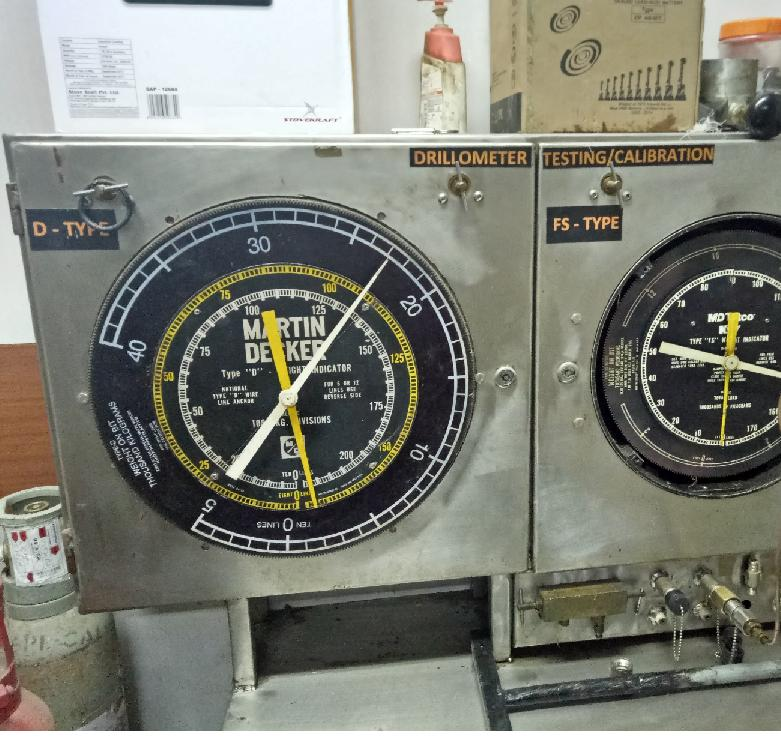
\includegraphics[scale=0.3]{images/drillometer}
\centering 
\caption{A Picture of Drillometer}
\end{figure}

 However, most rigs are equipped with a
weight indicator that has a second indicator dial that can be set to.
read zero ("zeroed") with the drill string hanging free, and works
backwards from the main indicator dial. After proper zeroing, any
weight set on bottom (that takes weight away from the main dial), has
the effect of adding weight to this secondary dial, so that the driller
can read weight on bit directly from the dial.